\documentclass[times, utf8, seminar]{fit}

\usepackage{verbatim}
%\batchmode
%\usepackage{booktabs}
\usepackage{listings}
\usepackage{longtable}
\usepackage{xcolor}
\usepackage{float}

\usepackage{hyperref}
\usepackage{graphicx}
\usepackage{etoolbox}
\usepackage{datetime}
\usepackage{needspace}
\usepackage[compact]{titlesec}
%\usepackage{hyperref}
%\titleformat{\chapter}[display]{\normalfont\huge\bfseries}{\chaptertitlename\ \thechapter}{20pt}{\Huge}

%http://stackoverflow.com/questions/3279194/remove-spacing-before-chapter-in-latex
%\usepackage{titlesec}
%\titleformat{\chapter}[display]
%{\normalfont\huge\bfseries}{\chaptertitlename\ \thechapter}{20pt}{\Huge}
% this alters "before" spacing (the second length argument) to 0
%\titlespacing*{\chapter}{0pt}{-20pt}{40pt}

%\renewcommand*{\chapterheadstartvskip}{\vspace*{0.5cm}}
%\renewcommand*{\chapterheadendvskip}{\vspace{1cm}}

% http://tex.stackexchange.com/questions/40436/vertical-space-before-section-title-with-titlesec

\usepackage[compact]{titlesec}
\usepackage{setspace}
\onehalfspacing

%\titleformat{\section}{\normalfont\bfseries}{\thesection}{1em}{}
%\titlespacing{\section}{0pt}{0pt}{0pt}

\usepackage{enumerate}
\usepackage[shortlabels]{enumitem}

\usepackage{underscore}

\begin{document}
\widowpenalty=300
\clubpenalty=300


\lstset{
  language=bash,
  backgroundcolor=\color{gray!25},
  basicstyle=\ttfamily \footnotesize,
  breaklines=true,
  prebreak=\raisebox{0ex}[0ex][0ex] {\ensuremath{\hookleftarrow}},
  columns=fullflexible,
  keywords={},
  mathescape=false
}



\title{Agilni \emph{software development},\newline test \& deployment}

\author{Ernad Husremović}
\brindex{DL 2792}
\verzija {0.0.5}

\mentor{mr. Adil Joldić}

\maketitle

\tableofcontents

%\listoftables
%\listoffigures
\newpage

\begin{abstract}

U ovom radu se na bazi konkretnog primjera\footnote{"HOWTO" stil} prezentuje infrastruktura za testiranje i instalaciju u produkcijskom okruženju (''test'' \& ''deploy'' infrastructure). Obradićemo instalaciju ''Gitlab'' servera koristeći sljedeće tehnologije i servise:
\begin{itemize}
  \item Github/git \url{https://github.com/hernad/gitlabhq}
  \item Vagrant  \url{http://vagrantup.com/}
  \item Chef opscode \url{http://www.opscode.com/chef}
  \item Rackspace cloud \url{http://www.rackspace.com/cloud}
\end{itemize}

\keywords{open source software, OSS, chef, vagrant, rackspace, git, github}
\end{abstract}

% abstract end

\chapter{Uvod}

%\vspace*{-1.2cm}
\section{Gitlab}
Gitlab je web servis koji obezbjeđuje upravljanje softverskim projektima. Gitlab obezbjeđuje sljedeće funkcije:
\begin{itemize}
  \item Git source code management - hostiranje izvornog koda unutar git repozitorija
  \item Issue management - elektronsko praćenje aktivnosti developera
  \item Milestone management - pojedine aktivnosti (issues) se mogu vezati uz odgovarajuću verziju (iteraciju) - ''milestone''
  \item Code snippets (code templates) - publikovanje uzoraka izvornog koda koje će tim koristiti
  \item Code/Commit review - komentarisanje izvornog koda
  \item Wikies - wikiji omogućavaju timski razvoj projektne dokumentacije
\end{itemize}

\section{Gitlab arhitektura}
''Gitlab'' je složen softverski sistem sastaljen od sljedećih komponenti:
\begin{enumerate}
  \item ubuntu linux server
  \item openssh server za razmjenu git repozitorija putem ssh protokola 
  \item ''nginx'' web server
  \item ''postfix'' email server
  \item ''ruby on rails'' framework je korišten za izradu web front-end-a.
  \item ''resque'' za background jobs \url{https://github.com/defunkt/resque}
  \item ''redis'' nosql (koristi ga ''resque'')
  \item ''mysql'' database backend\footnote{može se koristiti i postgresql}
  \item ''gitolite'' perl za upravljanje git repozitorijima
  \item ''pygments'' python ''source code higlighter''
\end{enumerate}

\section{''Devops'' metode}
Instalacija ovako složene infrastruktura traži značajno vrijeme i resurse za postavljanje testnog i produkcijskog okruženja. 
Agilni razvoj software-a potencira česte promjene i nadogradnje sistema. Testiranje i instalacija tih promjena u produkcijsko okruženje na konvencionalni način traži značajne resurse i vrijeme za realizaciju. Agilni pristup ovim zadacima potencira automatizaciju testnog i produkcijskog okruženje. Manuelne operacije se zamjenjuju atomatiziranim procedurama. Operacije instalacije i održavanja sistema se i same mogu posmatrati kao sofverski projekti.
Rezultat agilnog pristupa u segmentu instalacije i održavanja softverskog sistema je rezultirao ''Devops''\footnote{\url{http://en.wikipedia.org/wiki/DevOps}} metodama.

\section{Vagrant testno okruženje}

''Chef'' je dobar primjer ''devops'' alata. ''Chef'' recepti (''cookies'') sadrže programe kojim se instaliraju pojedine komponente sistema. Skup tih recepata definiše instalacijsku proceduru.

Naravno, produkcijskoj instalaciji sistema\footnote{instalaciji sistema namjenjenoj krajnjem kurisniku} predhodi testiranje.
''Vagrant'' je popularni alagt koji su ''devops'' pobornici prihvatili kao alat za izgradnju testnog okruženja. 
''Vagrant'' automatizira instaciju i kreiranje ''Virtual Box'' virtuelnih sesija\footnote{\url{https://www.virtualbox.org}}. Konfiguracija tih sesija se vrši uz pomoć ''chef configuration management'' sistema\footnote{može da se koristi i ''Puppet'' configuration managment sistem}.

\section{Instalacija testnog gitlab servera}

Preuzmimo vagrant\_gitlab projekat sa Github-a:

\$ \verb+git clone git://github.com/hernad/vagrant_gitlab.git+

Install skripta instalira sve potrebne ruby pakete koje će vagrant koristi\footnote{Naravno, prije toga je potrebno imati instalirano ''ruby'' programsko okruženje, preporučeno ''rvm'' ruby okruženje}, kao i sve ''cookbooks'' koje će koristiti ''chef'':

vagrant\_gitlab\$ \verb+./install.sh+

\verb+Vagrantfile+\footnote{\url{https://github.com/hernad/vagrant\_gitlab/blob/master/Vagrantfile}} sadrži konfiguraciju testnog gitlab servera. Vagrantfile nije ništa drugo nego ''ruby'' program. Konkretno, vagrant\_gitlab koristi niz sistemskih varijabli (OS environment)  kao parametre instalacije sistema\footnote{Parametri sadrže sve ono što su privatni podaci korisnika i što ne treba biti javno dostupno - imena hostova, korisnika, lozinke i sl.}

Komandom \verb+up.sh+ setujemo sistemske varijable, te kreiramo virutelnu sesiju:

vagrant\_gitlab\$ \verb+source up.sh+

\begin{lstlisting}
OS_AUTH_SYSTEM=rackspace
OS_AUTH_URL=https://identity.api.rackspacecloud.com/v2.0/
OS_DNS_DOMAIN=test.out.ba
OS_ENVARS='GMAIL_USER=bring.out.sa@gmail.com GMAIL_PASSWORD=pwd1 MYSQL_ROOT_PWD=pwd2 MYSQL_PWD=pwd3 GITHUB_USER=hernad GITHUB_PROJECT=vagrant_gitlab OS_SERVER_NAME=gitlab-stable.test.out.ba OS_DNS_DOMAIN=test.out.ba GITLAB_VERSION=v3.0.2 GITLAB_REPOS=git://github.com/hernad/gitlabhq.git'
OS_NO_CACHE=1
OS_PASSWORD=<rackspacecloud_api_key>
OS_PROJECT_ID=<rackspace_user>
OS_REGION_NAME=DFW
OS_SERVER_NAME=gitlab-stable.test.out.ba
OS_TENANT_NAME=bringout
OS_USERNAME=bringout
...
\end{lstlisting}

Nakon kreiranja gitlab ''VirtualBox'' testne sesije, slijedi pokretanje ''chef-solo''-a unutar sesije. ''chef-solo'' je zadužen za instalaciju i konfiguraciju testne sesije:

vagrant\_gitlab\$ \verb+source ./up.sh+
\begin{lstlisting}
[default] Clearing any previously set forwarded ports...
[default] Forwarding ports...
[default] -- 22 => 2222 (adapter 1)
[default] Creating shared folders metadata...
...
[default] Waiting for VM to boot. This can take a few minutes. <<<<<<< virtualbox sesija kreirana
[default] VM booted and ready for use!
[default] Detected Virtualbox Guest Additions 4.2.4 --- OK.
[default] Configuring and enabling network interfaces...
[default] Mounting shared folders...
[default] -- v-root: /vagrant
[default] -- v-csc-1: /tmp/vagrant-chef-1/chef-solo-1/cookbooks
[default] Running provisioner: Vagrant::Provisioners::ChefSolo...
[default] Generating chef JSON and uploading...
[default] Running chef-solo... <<<<<<<<<<< Pokrece se chef-solo na virtualbox sesiji
stdin: is not a tty
[Mon, 19 Nov 2012 11:33:15 +0000] INFO: *** Chef 0.10.10 ***
[Mon, 19 Nov 2012 11:33:15 +0000] INFO: Setting the run_list to ["recipe[build-essential]", "recipe[rvm::system]", "recipe[mysql::client]", "recipe[mysql::ruby]", "recipe[postgresql::client]", "recipe[postgresql::ruby]", "recipe[gitlab::default]", "recipe[gitlab::nginx]", "recipe[gitlab::database]"] from JSON
[Mon, 19 Nov 2012 11:33:15 +0000] INFO: Run List is [recipe[build-essential], recipe[rvm::system], recipe[mysql::client], recipe[mysql::ruby], recipe[postgresql::client], recipe[postgresql::ruby], recipe[gitlab::default], recipe[gitlab::nginx], recipe[gitlab::database]]
[Mon, 19 Nov 2012 11:33:15 +0000] INFO: Run List expands to [build-essential, rvm::system, mysql::client, mysql::ruby, postgresql::client, postgresql::ruby, gitlab::default, gitlab::nginx, gitlab::database]
[Mon, 19 Nov 2012 11:33:15 +0000] INFO: Starting Chef Run for precise32
...
[Mon, 19 Nov 2012 11:36:20 +0000] INFO: Processing package[ssl-cert] action install (/tmp/vagrant-chef-1/chef-solo-1/cookbooks/rvm/providers/ruby.rb line 156)
[Mon, 19 Nov 2012 11:36:22 +0000] INFO: package[ssl-cert] installed version 1.0.28ubuntu0.1
[Mon, 19 Nov 2012 11:36:22 +0000] INFO: Building rvm_ruby[ruby-1.9.3-p327], this could take awhile...
...
[Mon, 19 Nov 2012 14:18:58 +0000] INFO: Processing service[nginx] action reload (nginx::default line 39)
[Mon, 19 Nov 2012 14:18:58 +0000] INFO: service[nginx] reloaded
[Mon, 19 Nov 2012 14:18:58 +0000] INFO: template[/etc/init.d/gitlab] sending enable action to service[gitlab] (delayed)
[Mon, 19 Nov 2012 14:18:58 +0000] INFO: Processing service[gitlab] action enable (gitlab::default line 183)
[Mon, 19 Nov 2012 14:18:58 +0000] INFO: Chef Run complete in 994.730999 seconds
[Mon, 19 Nov 2012 14:18:58 +0000] INFO: Running report handlers
[Mon, 19 Nov 2012 14:18:58 +0000] INFO: Report handlers complete
\end{lstlisting}


\section{Gitlab merge from upstream}

\setlength{\parindent 0cm}
gitlabhq\$ \verb+git fetch gitlabhq+
\begin{lstlisting}
remote: Counting objects: 570, done.
remote: Compressing objects: 100\% (174/174), done.
remote: Total 342 (delta 262), reused 237 (delta 165)
Receiving objects: 100\% (342/342), 43.70 KiB, done.
Resolving deltas: 100\% (262/262), completed with 122 local objects.
From git://github.com/gitlabhq/gitlabhq
   dd4d124..3c7806c  master     -> gitlabhq/master
\end{lstlisting}

gitlabhq\$ \verb+git branch -l+
\begin{lstlisting}
* master
\end{lstlisting}


gitlabhq\$ \verb+git commit -a+
\begin{lstlisting}
[master 9bacff4] http://www.quora.com/Ruby-on-Rails/What-is-schema-rb-in-rails-project
 1 file changed, 19 insertions(+), 19 deletions(-)
\end{lstlisting}


gitlabhq\$ \verb+git diff HEAD^1 HEAD+
\begin{lstlisting}
diff --git a/db/schema.rb b/db/schema.rb
index 51ab207..19eb8eb 100644
--- a/db/schema.rb
+++ b/db/schema.rb
@@ -69,8 +69,8 @@ ActiveRecord::Schema.define(:version => 20121026114600) do
     t.boolean  "closed",                              :default => false, :null => false
     t.datetime "created_at",                                             :null => false
     t.datetime "updated_at",                                             :null => false
-    t.text     "st_commits",    :limit => 2147483647
-    t.text     "st_diffs",      :limit => 2147483647
+    t.text     "st_commits",    :limit => 4294967295

  ...

     t.integer  "project_id"
     t.string   "attachment"
     t.string   "line_code"
@@ -156,30 +156,30 @@ ActiveRecord::Schema.define(:version => 20121026114600) do
   end
 
   create_table "users", :force => true do |t|
\end{lstlisting}


gitlabhq\$ \verb+git merge gitlabhq/master+
\begin{lstlisting}
Removing lib/gitlab/encode.rb
Removing gitlab
Auto-merging doc/development.md
Removing Procfile.production
Merge made by the recursive strategy
 .travis.yml                                        |    2 +-
 CHANGELOG                                          |    2 +-
 Gemfile                                            |    4 +-
 Gemfile.lock                                       |   12 +++-
 Procfile.production                                |    2 -
 VERSION                                            |    2 +-
 app/assets/images/event_filter_comments.png        |  Bin 0 -> 750 bytes
 app/assets/images/event_filter_merged.png          |  Bin 0 -> 463 bytes
 app/assets/images/event_filter_push.png            |  Bin 0 -> 632 bytes
 
 ...

 app/controllers/application_controller.rb          |    9 +++
 app/controllers/blob_controller.rb                 |   10 +--
 app/controllers/dashboard_controller.rb            |   11 ++-
 app/controllers/profile_controller.rb              |    2 +-

 ...

 app/views/blame/show.html.haml                     |    4 +-
 app/views/commits/_commit.html.haml                |    4 +-
 app/views/commits/_head.html.haml                  |    5 ++
 app/views/dashboard/index.html.haml                |    9 ++-
 
 ... 
 
 delete mode 100644 Procfile.production
 create mode 100644 app/assets/images/event_filter_comments.png
 create mode 100644 app/assets/images/event_filter_merged.png
 create mode 100644 app/assets/images/event_filter_push.png
 ...
 delete mode 100644 lib/gitlab/encode.rb
 create mode 100644 lib/gitlab/git_stats.rb
 create mode 100644 vendor/assets/javascripts/g.bar-min.js
 create mode 100644 vendor/assets/javascripts/g.raphael-min.js
\end{lstlisting}

gitlabhq\$ \verb+git push origin master+

\begin{lstlisting}
Counting objects: 581, done.
Delta compression using up to 8 threads.
Compressing objects: 100\% (85/85), done.
Writing objects: 100\% (350/350), 45.00 KiB, done.
Total 350 (delta 267), reused 342 (delta 262)
To git@github.com:hernad/gitlabhq.git
   038ac96..28f5807  master -> master
\end{lstlisting}

\begin{figure}[H]
\centering
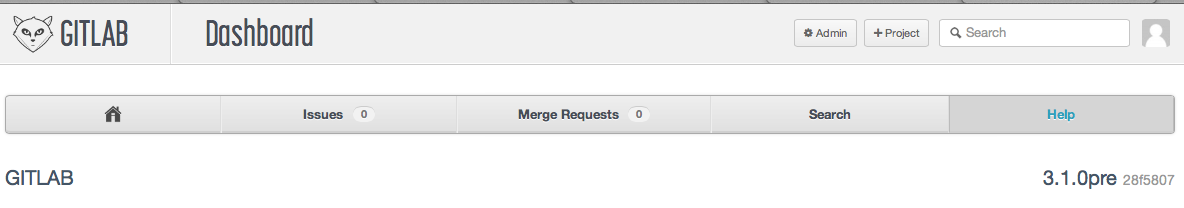
\includegraphics[width=15cm]{img/gitlab_hernad_310_after_merge.png}
\caption{Gitlabhq nakon `merge' operacije sa `upstream' projektom}
\end{figure}

\begin{figure}[H]
\centering
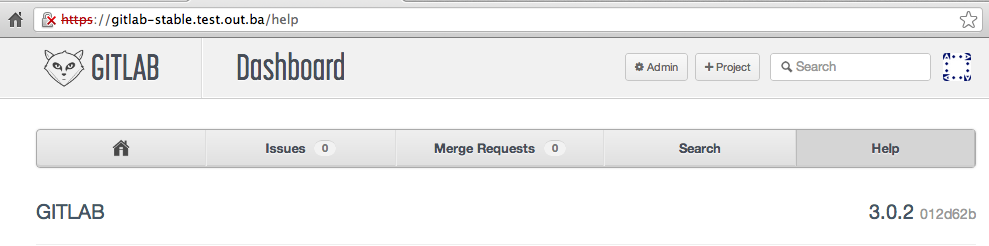
\includegraphics[width=15cm]{img/gitlab_stable_3.0.2.png}
\caption{Gitlabhq - stable 3.0.2}
\end{figure}


\begin{figure}[H]
\centering
\includegraphics[width=15cm]{img/gitlabhq_3.0.3.png}
\caption{Gitlabhq - 3.0.3}
\end{figure}


\chapter{Instalacija gitlab-a na rackspace cloud server}

\begin{lstlisting}
Server sa imenom gitlab.knowhow.out.ba vec postoji !
Server: gitlab.knowhow.out.ba IP: 198.101.149.48
server je kreiran !
Server: gitlab.knowhow.out.ba IP: 198.101.149.48
vrsim update domena knowhow.out.ba, zapis gitlab.knowhow.out.ba sa javnom adresom 198.101.149.48
./manage_domains.py -d knowhow.out.ba -r gitlab.knowhow.out.ba -i 198.101.149.48
dns_domain: knowhow.out.ba dns_record: gitlab.knowhow.out.ba ip_address 198.101.149.48

....

[2012-11-12T11:15:43+00:00] INFO: template[/etc/rvmrc] mode changed to 644
[2012-11-12T11:15:43+00:00] INFO: Processing execute[install system-wide RVM] action run (rvm::system_install line 76)
[2012-11-12T11:15:43+00:00] INFO: Processing execute[upgrade system-wide RVM to none] action run (rvm::system_install line 110)
[2012-11-12T11:15:43+00:00] INFO: Processing rvm_ruby[ruby-1.9.3-p327] action install (rvm::system line 170)
/root/vagrant_gitlab/cookbooks/rvm/libraries/rvm_chef_user_environment.rb:36: warning: class variable access from toplevel
[2012-11-12T11:15:45+00:00] INFO: Processing package[build-essential] action install (/root/vagrant_gitlab/cookbooks/rvm/providers/ruby.rb line 156)
[2012-11-12T11:15:45+00:00] INFO: Processing package[openssl] action install (/root/vagrant_gitlab/cookbooks/rvm/providers/ruby.rb line 156)
[2012-11-12T11:15:45+00:00] INFO: Processing package[libreadline6] action install (/root/vagrant_gitlab/cookbooks/rvm/providers/ruby.rb line 156)
[2012-11-12T11:15:45+00:00] INFO: Processing package[libreadline6-dev] action install (/root/vagrant_gitlab/cookbooks/rvm/providers/ruby.rb line 156)
[2012-11-12T11:15:45+00:00] INFO: Processing package[zlib1g] action install (/root/vagrant_gitlab/cookbooks/rvm/providers/ruby.rb line 156)
[2012-11-12T11:15:45+00:00] INFO: Processing package[zlib1g-dev] action install (/root/vagrant_gitlab/cookbooks/rvm/providers/ruby.rb line 156)
[2012-11-12T11:15:45+00:00] INFO: Processing package[libssl-dev] action install (/root/vagrant_gitlab/cookbooks/rvm/providers/ruby.rb line 156)
[2012-11-12T11:15:45+00:00] INFO: Processing package[libyaml-dev] action install (/root/vagrant_gitlab/cookbooks/rvm/providers/ruby.rb line 156)

...

[2012-11-12T11:15:45+00:00] INFO: Processing package[libsqlite3-dev] action install (/root/vagrant_gitlab/cookbooks/rvm/providers/ruby.rb line 156)
[2012-11-12T11:15:45+00:00] INFO: Processing package[sqlite3] action install (/root/vagrant_gitlab/cookbooks/rvm/providers/ruby.rb line 156)
[2012-11-12T11:15:46+00:00] INFO: Processing package[libxml2-dev] action install (/root/vagrant_gitlab/cookbooks/rvm/providers/ruby.rb line 156)
[2012-11-12T11:15:46+00:00] INFO: Processing package[libxslt-dev] action install (/root/vagrant_gitlab/cookbooks/rvm/providers/ruby.rb line 156)
[2012-11-12T11:15:46+00:00] INFO: package[libxslt-dev] is a virtual package, actually acting on package[libxslt1-dev]
[2012-11-12T11:15:46+00:00] INFO: Processing package[autoconf] action install (/root/vagrant_gitlab/cookbooks/rvm/providers/ruby.rb line 156)
[2012-11-12T11:15:46+00:00] INFO: Processing package[libc6-dev] action install (/root/vagrant_gitlab/cookbooks/rvm/providers/ruby.rb line 156)
[2012-11-12T11:15:46+00:00] INFO: Processing package[ncurses-dev] action install (/root/vagrant_gitlab/cookbooks/rvm/providers/ruby.rb line 156)
[2012-11-12T11:15:46+00:00] INFO: package[ncurses-dev] is a virtual package, actually acting on package[libncurses5-dev]
[2012-11-12T11:15:46+00:00] INFO: Processing package[automake] action install (/root/vagrant_gitlab/cookbooks/rvm/providers/ruby.rb line 156)
[2012-11-12T11:15:46+00:00] INFO: Processing package[libtool] action install (/root/vagrant_gitlab/cookbooks/rvm/providers/ruby.rb line 156)
[2012-11-12T11:15:46+00:00] INFO: Processing package[bison] action install (/root/vagrant_gitlab/cookbooks/rvm/providers/ruby.rb line 156)
[2012-11-12T11:15:46+00:00] INFO: Processing package[ssl-cert] action install (/root/vagrant_gitlab/cookbooks/rvm/providers/ruby.rb line 156)
[2012-11-12T11:15:47+00:00] INFO: Building rvm_ruby[ruby-1.9.3-p327], this could take awhile...

....

boostrap chef for vagrant_gitlab is finished (0.9.9) :)
restartujem server ...
Restartujem server gitlab.knowhow.out.ba

real15m29.472s
user0m3.928s
sys0m0.387s
\end{lstlisting}

root@gitlab:~# \verb+sudo su - www-data+
\begin{lstlisting}
www-data@gitlab:~\$ cd /opt/gitlab
Using /usr/local/rvm/gems/ruby-1.9.3-p327
Using ruby-1.9.3-p327 with gemset gitlab
Using /usr/local/rvm/gems/ruby-1.9.3-p327 with gemset gitlab
\end{lstlisting}


www-data@gitlab:/opt/gitlab\$ \verb+cat /etc/init.d/gitlab | grep ruby+
\begin{lstlisting}
source "/usr/local/rvm/environments/ruby-1.9.3-p327"
declare -r GITLAB_RUBY="ruby-1.9.3-p327@gitlab"
\end{lstlisting}

\end{document}
